\chapter{Résultats de simulation et analyse du modèle à état discret}
\label{ch:simu}

Afin de valider les constats émis au chapitre \ref{ch:modele_discret}, cette partie se propose d'effectuer des simulations numériques afin d'étudier la stabilité des différents points d'équilibre.

Pour ce faire, ce chapitre se consacre à l'analyse de bifurcation, comme déjà utilisée dans \cite{ChaosControl}. Le code fourni en complément du rapport est fortement basé sur le tutoriel d'analyse de bifurcation pour Python présenté en \cite{bifurc} avec l'exemple de l'équation logistique.

\section{Obtention du diagramme de bifurcation}
\label{sec:diagramme_bifurcation}

Afin d'obtenir un diagramme de bifurcation, il a fallu décider d'un paramètre pertinent à faire varier et choisir les valeurs auxquelles fixer tous les autres paramètres. En repartant de l'équation logistique présentée dans \cite{bifurc}, nous avons décidé de faire varier le paramètre $\alpha$, mais aussi d'imposer les deux conditions suivantes :
\begin{itemize}
	\item $\gamma = \alpha$ comme dans l'équation logistique ;
	\item $\beta = 0.1 \alpha$, car plus les proies se reproduisent vite, plus la probabilité qu'un prédateur chasse une proie avec succès est grande.
\end{itemize}

Mathématiquement, le diagramme de bifurcation revient à chercher les valeurs d'adhérence des deux suites $(x_n)$ et $(y_n)$. Pour cela, le programme proposé en complément de ce rapport calcule $1000$ itérations du système \ref{eq:syst_discret} pour chaque valeur de $\alpha$ et affiche les $100$ dernières valeurs obtenues. Pour une configuration stable, les simulations effectuées avec tous les paramètres fixés (voir figure \ref{fig:simu param fixes}) nous montrent que le système se stabilise avant la $900$ème itération, ce qui assure l'obtention de valeurs cohérentes.

\section{Analyse de la simulation}
\label{sec:analyse_simu}

Afin d'analyser les résultats obtenus à la figure \ref{fig:bifurc}, on peut comparer les conditions de stabilité mises en lumière sur le diagramme de bifurcation avec les conditions de stabilités sur les valeurs propres du linéarisé tangent à l'équilibre $(x^*, y^*)$, comme décrit en (\ref{eq:matrices equilibre}).

Par lecture graphique, on trouve que la valeur limite de bifurcation est $\alpha = 2.2$. Vérifions par le calcul la pertinence de cette valeur par rapport au modèle théorique.

Après calculs (menés dans la seconde partie du fichier $`Diagramme\_Bifurcation.py`$), on obtient tout d'abord comme valeurs pour $x^*$ et $y^*$ les valeurs suivantes : $x^* = 0.894$ et $y^* = 2.904$, ce qui est cohérent avec ce que l'on observe sur le diagramme de bifurcation aux alentours de $\alpha = 2.2$.

Ensuite, on cherche à vérifier que le point $\alpha = 2.2$ est un point critique pour la stabilité de l'équilibre $(x^*, y^*)$. Pour cela, on applique le critère de Jury avec l'ensemble des paramètres fixés. Cependant, les calculs à la fois du critère de Jury et de l'obtention des valeurs propres de la matrice linéarisée tangent avec le module numpy indiquent que l'équilibre est sensé être instable.

En effet, on obtient comme valeurs propres pour la matrice :
\begin{equation}
	\label{eq:matrice tangente en x*,y*}
	J_{2}(x^*, y^*) = 
  	\begin{bmatrix}
    	1 - \alpha + \beta y^* & - \beta x^* \\
    	\sigma y^* & 1 - \rho + \sigma x^* + 2 \nu y^*
  	\end{bmatrix}
	\text{(déja vue au chapitre \ref{ch:modele_discret})}
\end{equation}
les deux valeurs propres suivantes $\lambda_1 = -0.94668619$ et $\lambda_2 = 1.33001952$. Or on a $|\lambda_2| > 1$, donc le système devrait être instable, ce qui ne correspond pas au résultat de la simulation en figure \ref{fig:simu param fixes}, effectuée avec les mêmes paramètres que les calculs précédents.

Une explication possible à cette contradiction entre le calcul théorique et la simulation est peut-être la différence entre l'étude du système linéarisé tangent au point d'équilibre à travers la matrice \ref{eq:matrice tangente en x*,y*} et l'étude du véritable système non-linéaire \ref{eq:syst_discret}. En effet, le passage à la jacobienne implique une perte d'information qui pourrait expliquer la différence entre les résultats théoriques et la simulation.



\begin{figure}
    \begin{center}
		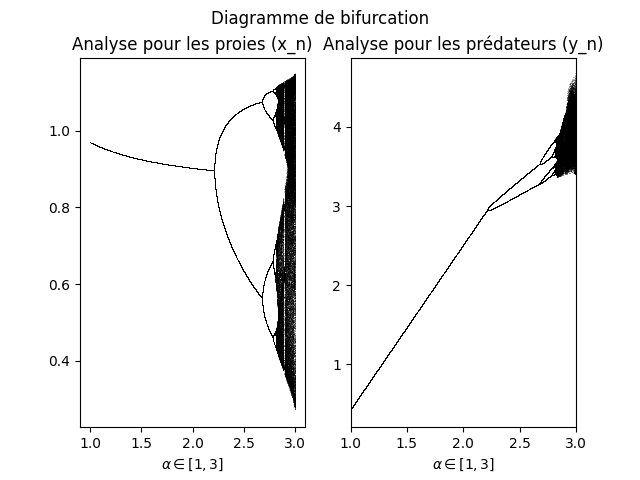
\includegraphics[height=7cm]{figures/Bifurcation_1.png}
	\end{center}
	\caption{Analyse de bifurcation pour les paramètres $\alpha \in [1, 3]$; $\beta = 0.08$; $\gamma = \alpha$; $\rho = 0.08$; $\sigma = 0.1 \alpha$ et $\nu = 0.04$ avec les conditions initiales $x_0 = 1.1$ et $y_0 = 1$}
    \label{fig:bifurc}
\end{figure}

\begin{figure}
    \begin{center}
		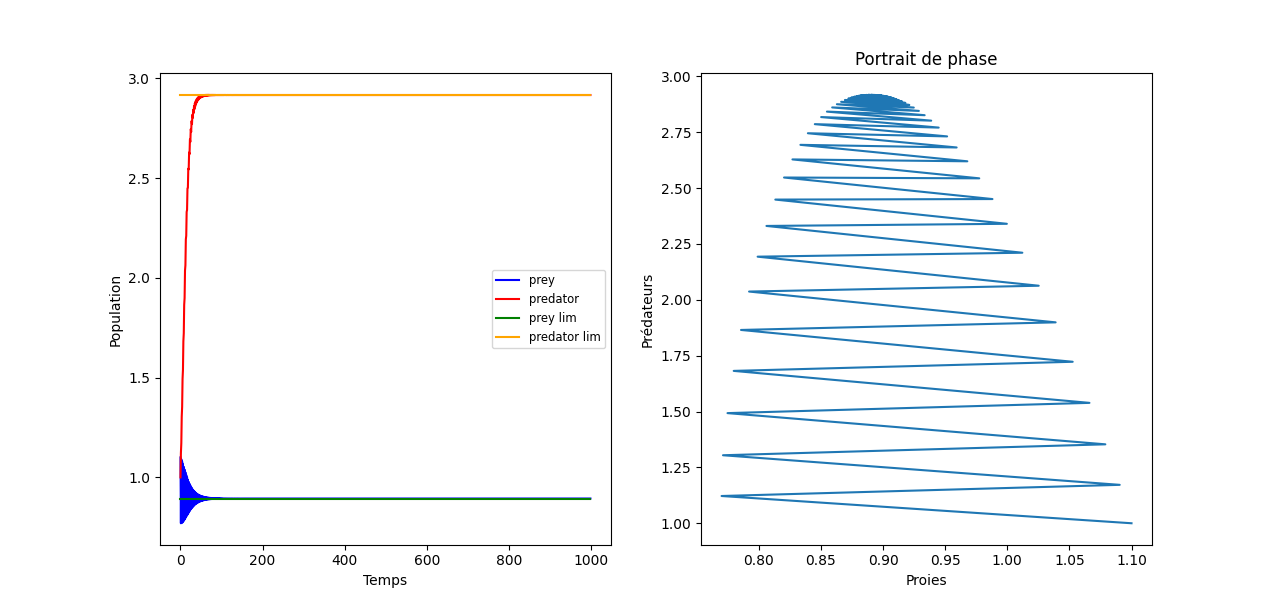
\includegraphics[height=7cm]{figures/Simu_1.png}
	\end{center}
	\caption{Simulation du système pour les paramètres $\alpha = 2.2$; $\beta = 0.08$; $\gamma = \alpha = 2.2$; $\rho = 0.08$; $\sigma = 0.1 \alpha = 0.22$ et $\nu = 0.04$ avec les conditions initiales $x_0 = 1.1$ et $y_0 = 1$}
    \label{fig:simu param fixes}
\end{figure}